\documentclass{article}
\pagestyle{empty}
\usepackage{amsmath,amssymb}
\usepackage{xcolor}
\usepackage{tikz}
\usetikzlibrary{arrows.meta,positioning,fit,calc,backgrounds}

\newcommand{\GS}{\mathrm{GS}}
\newcommand{\dhatmax}{\hat{d}_{\max}}
\newcommand{\Lap}{\mathrm{Lap}}

\newsavebox{\figbox}
\newcommand{\fs}{\fontsize{6}{7}\selectfont}

\begin{document}
\savebox{\figbox}{%
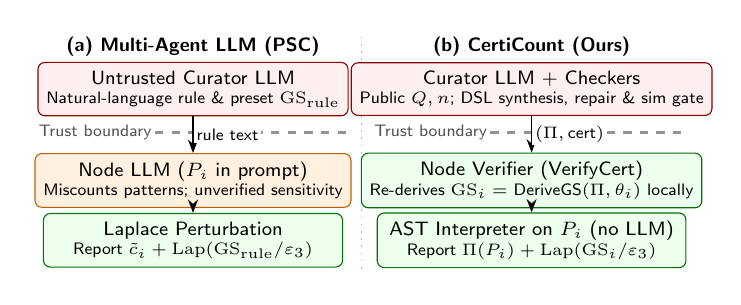
\begin{tikzpicture}[
    font=\sffamily\scriptsize,
    box/.style={draw, rounded corners=2.5pt, align=center, inner sep=3pt, minimum height=15pt},
    untrusted/.style={box, fill=red!6, draw=red!55!black},
    llmnode/.style={box, fill=orange!12, draw=orange!75!black},
    trusted/.style={box, fill=green!7, draw=green!45!black},
    arr/.style={-{Stealth[scale=0.85]}, semithick}
]
% Inner padding box for clean crop
\path (-4.22, -0.82) rectangle (4.32, 2.32);

% Left panel: PSC
\node[font=\sffamily\scriptsize\bfseries] at (-2.12, 2.10) {(a) Multi-Agent LLM (PSC)};
\node[untrusted, minimum width=3.80cm] (p_cur) at (-2.12, 1.56) {Untrusted Curator LLM\\[-1pt]{\fs Natural-language rule \& preset $\GS_{\mathrm{rule}}$}};
\draw[dashed, gray!85, thick] (-4.08, 1.01) -- (-0.16, 1.01);
\node[font=\sffamily\fs, text=gray!65!black, fill=white, inner sep=1pt, anchor=west] at (-4.12, 1.01) {Trust boundary};
\node[llmnode, minimum width=3.80cm] (p_node) at (-2.12, 0.40) {Node LLM ($P_i$ in prompt)\\[-1pt]{\fs Miscounts patterns; unverified sensitivity}};
\node[trusted, minimum width=3.80cm] (p_lap) at (-2.12, -0.36) {Laplace Perturbation\\[-1pt]{\fs Report $\tilde{c}_i + \Lap(\GS_{\mathrm{rule}}/\varepsilon_3)$}};
\draw[arr] (p_cur) -- node[right, font=\sffamily\fs, fill=white, inner sep=1pt]{rule text} (p_node);
\draw[arr] (p_node) -- (p_lap);

% Subtle vertical separator
\draw[dotted, gray!60, semithick] (0.02, -0.72) -- (0.02, 2.22);

% Right panel: CertiCount
\node[font=\sffamily\scriptsize\bfseries] at (2.18, 2.10) {(b) \textsc{CertiCount} (Ours)};
\node[untrusted, minimum width=3.92cm] (c_cur) at (2.18, 1.56) {Curator LLM + Checkers\\[-1pt]{\fs Public $Q, n$; DSL synthesis, repair \& sim gate}};
\draw[dashed, gray!85, thick] (0.18, 1.01) -- (4.18, 1.01);
\node[font=\sffamily\fs, text=gray!65!black, fill=white, inner sep=1pt, anchor=west] at (0.14, 1.01) {Trust boundary};
\node[trusted, minimum width=3.92cm] (c_ver) at (2.18, 0.40) {Node Verifier ($\mathsf{VerifyCert}$)\\[-1pt]{\fs Re-derives $\GS_i = \mathsf{DeriveGS}(\Pi, \theta_i)$ locally}};
\node[trusted, minimum width=3.92cm] (c_exe) at (2.18, -0.36) {AST Interpreter on $P_i$ (no LLM)\\[-1pt]{\fs Report $\Pi(P_i) + \Lap(\GS_i/\varepsilon_3)$}};
\draw[arr] (c_cur) -- node[right, font=\sffamily\fs, fill=white, inner sep=1pt]{$(\Pi, \mathsf{cert})$} (c_ver);
\draw[arr] (c_ver) -- (c_exe);
\end{tikzpicture}%
}%
\pdfpagewidth=\wd\figbox
\pdfpageheight=\dimexpr\ht\figbox+\dp\figbox\relax
\hoffset=-1in
\voffset=-1in
\topmargin=0pt \headheight=0pt \headsep=0pt \oddsidemargin=0pt \evensidemargin=0pt
\parindent=0pt
\vbox to \pdfpageheight{\hbox to \pdfpagewidth{\usebox{\figbox}}\vss}
\end{document}
